\documentclass{article}
\usepackage{graphicx}
% set font encoding for PDFLaTeX or XeLaTeX
\usepackage{ifxetex}
\ifxetex
  \usepackage{fontspec}
\else
  \usepackage[T1]{fontenc}
  \usepackage[utf8]{inputenc}
  \usepackage{lmodern}
\fi

% used in maketitle
\title{Atmósfera de la Tierra}
\author{Roberto Alexis Gómez Pintor}

% Enable SageTeX to run SageMath code right inside this LaTeX file.
% documentation: http://mirrors.ctan.org/macros/latex/contrib/sagetex/sagetexpackage.pdf
% \usepackage{sagetex}

\begin{document}
\maketitle
\section{Introducción}
La atmósfera de la Tierra  esta compuesta por una serie de gases, conocido normalmente como aire, esta atmósfera rodea la Tierra siendo retenida por la gravedad del mismo planeta. La misma atmósfera permite que exista vida en la Tierra y crea una presión haciendo que se forme agua líquida, tambien esta atmósfera protege al absorber la radiación ultravioleta, retener el calor y reducciendo las temperaturas durante el dia y noche. Esta atmósfera esta compuesta de varios elementos en volumen, el aire seco contiene 78.09\% de nitrogeno, 20.95\% de oxigeno, 0.93\% de argon, 0.04\% de dioxido de carbono y pequeñas cantidades de otros gases. La atmósfera tiene una masa de 5.15x10\textasciicircum{18}kg, el contenido de aire y la presión atmosférica varían en las diferentes capas, y el aire adecuado para su uso en la fotosíntesis por plantas terrestres y la respiración de animales terrestres se encuentra solo en la troposfera terrestre y en atmósferas artificiales.

\begin{figure}
  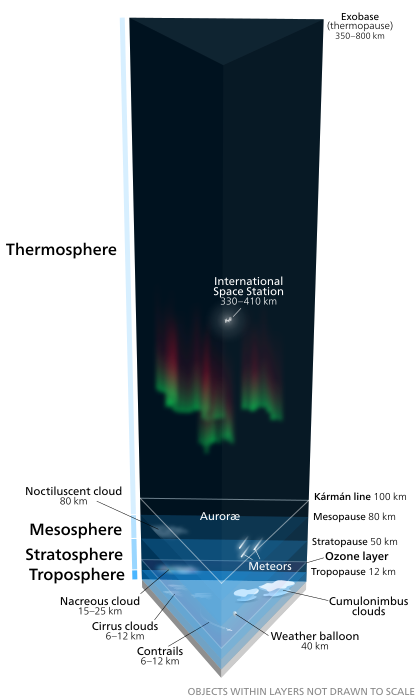
\includegraphics[width=\linewidth]{caps.png}
  \caption{Vista de las capas}
  \label{fig:boat1}
\end{figure}
\section{Composicion}
Los principales componentes en la atmósfera nitrogeno, oxigeno y el argón, tambien tiene compuesto de vapor de agua que representa el 0.25\% de la masa de la atmósfera y tiene una concentraccion que varia alrededor de 10 ppm de volume. Los otros gases aveces llamados gases rezagados cuales se encuentra los gases del efecto invernadero como el dioxido de carbono, metano, oxido nitroso y el ozono, aunque tambien estan presentes otros gases derivados tanto de forma natural como cenizas volcanicas, polen, esporas y brisa marina. Tambien pueden estar contaminantes producto de la industria como cloro y compuestos de azufre.

\section{Estructura de la atmósfera}
\subsection{capas principales}
En general, la presión del aire y la densidad disminuyen con la altitud en la atmósfera. Sin embargo, la temperatura tiene un perfil más complicado con la altitud, y puede permanecer relativamente constante o incluso aumentar con la altitud en algunas regiones, esto influye en que la temperatura y la altitud sean 2 factores constantemente vigilados, sobretodo la temperatura que nos permite dividir la atmosfera en una clasificacion llamada estratificacion atmosferica. Estas capas son 5 en total, aunque la exosfera se le excluye, las 4 principales son  troposfera, la estratosfera, la mesosfera y la termosfera, que van de mayor a menor tamaño.

Exosfera 700-10,000 km, termosfera 80-700 km, mesosfera 50-80 km, estratosfera 12-50 km, y troposfera 0-12 km.

\subsubsection{Exosfera}
La capa mas externa de la atmosfera de la Tierra se inicia desde los limites de la termosfera inicia a 700 km hasta los 10,000 km de altitud sobre el nivel del mar donde estan los vientos solares. Esta compuesta por varias densidades aunque muy bajascomo el hidrogeno y helio. En esta capa existen atomos y moleculas que estan separadas entre si haciendo que puedan moverse por ciendos de kilometros sin colosionar entre ellas. En esta capa habitan la mayoria de los satelites artificiales que orbitan el planeta.

\subsubsection{Termosfera}
La termosfera es la segunda capa mas alta desde los 80 km hasta los 700 km de altitud,esta capa tiene la temperatura de aumento constantpuede llegar hasta los $1,500^{\circ}$C aunque las moléculas de gas están tan separadas que su temperatura en el sentido habitual no es muy significativa. El aire está tan enrarecido que una molécula individual viaja un promedio de 1 km entre choques con otras moleculas. En esta capa esta libre de vapor aunque eso no quiere decir que no ocurran otros fenomenos no hidrometereologicos como aurora boreal y aurora astral, ademas la estacion espacial internacional orbita en esta capa entre 350 y 420 km.

\subsubsection{Mesosfera}
Es la tercera capa de la atmósfera tiene su altitud  de 50-80km estando entre el inicio de la termosfera y al final de la estratosfera, las temperaturas en esta capa son muy bajas llegando hasta los $-85^{\circ}$C el vapor de agua es muy escaso debido al aire frio de la misma capa. Estas son las nubes más altas en la atmósfera y pueden ser visibles a simple vista si la luz del sol se refleja en ellas una o dos horas después de la puesta del sol o un período de tiempo similar antes del amanecer. Esta capa es tambien donde los meteoritos se queman al entrar en la atmósfera, esta capa esta muy alta para ser alcanzada por vehiculos aereos normales como aviones y dirigibles, tambien esta muy debajo para el uso de naves espaciales y cohetes orbitales.

\subsubsection{Estatrosfera}
La estratosfera es la segunda capa más baja de la atmósfera de la Tierra. Se encuentra por encima de la troposfera y está separada de ella por la tropopausa. La presión atmosférica en la parte superior de la estratosfera es aproximadamente 1/1000 de la presión al nivel del mar. Contiene la capa de ozono, que es la parte de la atmósfera de la Tierra que contiene concentraciones relativamente altas de ese gas, esta capa tiene un aumento de temperatura relacionado con su altitud. El perfil de temperatura estratosférico crea condiciones atmosféricas muy estables, por lo que la estratosfera carece de la turbulencia del aire que produce el clima y que prevalece en la troposfera. En consecuencia, la estratosfera está casi completamente libre de nubes y otras formas de clima, tambien es la capa limite que puede los aviones de reaccion llegar.
\subsubsection{Troposfera}
La troposfera es la capa más baja de la atmósfera de la Tierra. Se extiende desde la superficie de la Tierra a una altura promedio de aproximadamente 12 km, aunque esta altitud varía de unos 9 km en el ecuador mientras que los polos llega a 17 km. Aunque se producen variaciones, la temperatura generalmente disminuye con el aumento de la altitud en la troposfera porque la troposfera se calienta principalmente a través de la transferencia de energía desde la superficie. Por lo tanto, la parte más baja de la troposfera (es decir, la superficie de la Tierra) es típicamente la sección más cálida de la troposfera. Casi todo el vapor de agua atmosférico o humedad se encuentra en la troposfera, por lo que es la capa donde tiene lugar la mayor parte del clima de la Tierra. Básicamente, tiene todos los tipos de nubes nubladas asociadas al clima generadas por la circulación activa del viento, aunque las nubes de trueno cumulonimbus muy altas pueden penetrar la tropopausa desde abajo y subir a la parte inferior de la estratosfera.

\subsection{Otras capas}
En otras capas secundarias podemos entrar la capa de ozono, la ionosfera, hetereosfera, heterosfera y capa limite.
\subsubsection{Capa de ozono}
La capa de ozono está contenida dentro de la estratosfera. En esta capa, las concentraciones de ozono son aproximadamente de 2 a 8 partes por millón, que es mucho más alta que en la atmósfera más baja, aunque es muy pequeña en comparcion de otras capas. Alrededor del 90\% del ozono en la atmósfera de la Tierra está contenido en la estratosfera.
\subsubsection{Ionosfera}
La ionosfera es una región de la atmósfera ionizada por la radiación solar. Es responsable de auroras. Durante el día, se extiende de 50 a 1,000 km.  Tiene importancia práctica porque influye, por ejemplo, en la propagación de la radio en la Tierra
\subsubsection{Hetereosfera y Heterosfera}
La homósfera y la heterosfera se definen según si los gases atmosféricos están bien mezclados. La homosfera basada en la superficie incluye la troposfera, la estratosfera, la mesosfera y la parte más baja de la termosfera, donde la composición química de la atmósfera no depende del peso molecular porque los gases se mezclan por la turbulencia.
\subsubsection{Capa limite}

La capa límite planetaria es la parte de la troposfera más cercana a la superficie de la Tierra y directamente afectada por ella, principalmente a través de la difusión turbulenta. Durante el día, la capa límite planetaria suele estar bien mezclada, mientras que por la noche se estratifica de forma estable con una mezcla débil o intermitente.
\section{Propiedades fisicas}
\subsection{Presion y Espesor}
La presión atmosférica promedio a nivel del mar está definida por la Atmósfera Estándar Internacional como 101,325 pascales.  Esto a veces se conoce como una unidad de atmósferas estándar (atm). La masa atmosférica total es 5.1480\textasciicircum{18}Kg, aproximadamente 2.5\% menos de lo que se deduciría de la presión media del nivel del mar. La presión atmosférica es el peso total del aire sobre el área de la unidad en el punto donde se mide la presión. Por lo tanto, la presión del aire varía según la ubicación y el clima.
\subsection{Temperatura y velocidad del sonido}
La división de la atmósfera en capas principalmente por referencia a la temperatura se discutió anteriormente. La temperatura disminuye con la altitud comenzando al nivel del mar, pero las variaciones en esta tendencia comienzan por encima de los 11 km, donde la temperatura se estabiliza a través de una gran distancia vertical a través del resto de la troposfera. En la estratosfera, comenzando por encima de unos 20 km, la temperatura aumenta con la altura, debido al calentamiento dentro de la capa de ozono causado por la captura de radiación ultravioleta significativa del Sol por el dioxígeno y el gas ozono en esta región. Debido a que en un gas ideal de composición constante, la velocidad del sonido depende únicamente de la temperatura y no de la presión o densidad del gas, la velocidad del sonido en la atmósfera con la altitud adquiere la forma del perfil de temperatura complicado y no refleja los cambios altitudinales en densidad o presión.


\subsection {Masa y Densidad}

La densidad del aire a nivel del mar es de aproximadamente 1.2 kg / m3, la densidad no se mide directamente, aunque se calcula a partir de mediciones de temperatura, presión y humedad utilizando la ecuación de estado para el aire tomando la ida de que es un gas ideal. La masa promedio de la atmosfera es aproximadamente de 5x10\textasciicircum{15} de toneladas.
\section{Propiedades opticas}
\subsection{Dispercion}


Cuando la luz pasa a través de la atmósfera de la Tierra, los fotones interactúan con ella a través de la dispersión. Si la luz no interactúa con la atmósfera, se llama radiación directa y es lo que verá si mirara directamente al Sol. Debido a un fenómeno llamado dispersión de Rayleigh, las longitudes de onda más cortas (azules) se dispersan más fácilmente que las longitudes de onda más largas (rojas). Es por eso que el cielo se ve azul; estás viendo luz azul dispersa.  Esta es también la razón por la cual los atardeceres son rojos. Debido a que el Sol está cerca del horizonte, los rayos del Sol pasan a través de más atmósfera de lo normal para llegar a su ojo. Gran parte de la luz azul se ha dispersado, dejando la luz roja en una puesta de sol.
\subsection{Absorcion}
Diferentes moléculas absorben diferentes longitudes de onda de radiación. Por ejemplo, O2 y O3 absorben casi todas las longitudes de onda más cortas que 300 nanómetros. Un ejemplo como el agua absorbe muchas longitudes de onda por encima de los 700 nm
\subsection{Emision}
La emisión es lo opuesto a la absorción, es cuando un objeto emite radiación. Los objetos tienden a emitir cantidades y longitudes de onda de radiación dependiendo de sus curvas de emisión de "cuerpo negro", por lo tanto, los objetos más calientes tienden a emitir más radiación, con longitudes de onda más cortas. Los objetos más fríos emiten menos radiación, con longitudes de onda más largas. Debido a su temperatura, la atmósfera emite radiación infrarroja. Por ejemplo, en las noches despejadas, la superficie de la Tierra se enfría más rápido que en las noches nubladas.
\subsection{Indice de refraccion}

El índice de refracción del aire es cercano, pero apenas superior a 1. Las variaciones sistemáticas en el índice de refracción pueden conducir a la flexión de los rayos de luz en recorridos ópticos largos. Un ejemplo es que, en algunas circunstancias, los observadores a bordo de barcos pueden ver otras embarcaciones justo sobre el horizonte porque la luz se refracta en la misma dirección que la curvatura de la superficie de la Tierra. El índice de refracción del aire depende de la temperatura, dando lugar a efectos de refracción cuando el gradiente de temperatura es grande. Un ejemplo de tales efectos es el espejismo.
\section{Preguntas}
\subsection{¿Qué fue lo que más te llamó la atención de esta actividad?}
Aprender una forma para desarrollar textos sin el uso de alguna suite office, ademas para mejorar la calidad de informes y documentos en el trabajo.
\subsection{¿Qué fue lo que se te hizo menos interesante?}
Pues nomas en el uso constante del ingles y sus servicios que aunque son sencillos de entender una vez que son explicados, tambien es donde se trabaja debido a que a la lentitud de cargar cambios.
\subsection{¿Qué cambios harías para mejorar esta actividad?}
Pues no encuentro fallos significativos para hacer cambios.
\subsection{¿Cuál es tu primera impresión de uso de LATEX?}
Aprender otro lenguaje de programacion como FORTRAN.
\subsection{¿El tiempo sugerido para esta actividad fue suficiente?}
Pues es un termino medio de tiempo, no fue corto ni sumamente largo, me parece un tiempo de entrega bastante aceptable, dependiendo si el usuario tiene otros bajaos o no.
\subsection{¿Encontraste algún documento o recurso en línea útil que quisieras compartir con los demás?}
La verdad trabaje con la informacion que me daba la actividad.
\end{document}
